\documentclass[10pt,a4paper,oneside,twocolumn]{article}

    \usepackage{float}	% for floating figures (putting them anywhere we want
    \usepackage{amsmath}	% for maths
    \usepackage{graphicx}	% jpg
    \usepackage{hyperref}
    \usepackage{textcomp}
    \usepackage{verbatim}	% use of \begin{comment}
    \usepackage{pgfplots}	% use of pgf plots
    \usepackage{multicol}
    \usepackage[top=2cm, bottom=2cm, left=1.5cm, right=1.5cm]{geometry} %margins
    \usepackage{sidecap}	% for side captions
    \restylefloat{table}	% floating figures(Tables)
    \usepackage{caption}
    \captionsetup{justification=centering}
    \usepackage{subcaption}
    \usepackage{array}

    \newcommand{\red}[1]{\textcolor{red}{#1}} 
    \newcommand{\cyan}[1]{\textcolor{cyan}{#1}} 
    \newcommand{\orange}[1]{\textcolor{orange}{#1}} 
    \newcommand{\purple}[1]{\textcolor{purple}{#1}} 
    \definecolor{forestgreen}{RGB}{0,102,0}
    \newcommand{\green}[1]{\textcolor{forestgreen}{#1}} 

    \numberwithin{equation}{section} %permits numbering within sections instead of globally
\begin{document}

\title{\huge{\textbf{Report}}\\
	\vspace{0.5cm}
	\Large{\textit{\'Ecole Polytechnique F\'ed\'erale de Lausanne, Switzerland}}}
\author{\large{Florian + Dariush}}

\begin{titlepage}
 \maketitle
\thispagestyle{empty}
\end{titlepage}

\section{Introduction}
    Introduction to the article goes here    Introduction to the article goes here  Introduction to the article goes here  Introduction to the article goes here  Introduction to the article goes here  Introduction to the article goes here  Introduction to the article goes here  Introduction to the article goes here  Introduction to the article goes here  Introduction to the article goes here  Introduction to the article goes here  Introduction to the article goes here  Introduction to the article goes here  Introduction to the article goes here  Introduction to the article goes here  Introduction to the article goes here  Introduction to the article goes here  Introduction to the article goes here  Introduction to the article goes here  Introduction to the article goes here  Introduction to the article goes here  Introduction to the article goes here Introduction to the article goes here \\

\section{The Model}

    \begin{figure*}[!h]
	\begin{subfigure}[b]{0.5\textwidth}
	    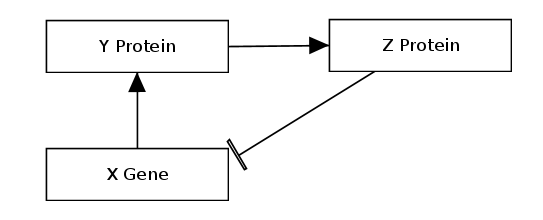
\includegraphics[width=\textwidth]{sketch.png}
	    \caption{
		One-Cell Model\\
	    The gene $X$ codes for protein $Y$ which, in turn, activates transcriptional inhibitor $Z$. The resulting model behaves as a three-variable oscillator.
	    }
	\end{subfigure}
	~
	\begin{subfigure}[b]{0.5\textwidth}
	    \begin{equation*}\frac{\delta X}{\delta t} = v_1 \frac{K_1^n}{K_1^n + Z^n} - v_2 \frac{X}{K_2 + X} \end{equation*}
	    \begin{equation*}\frac{\delta Y}{\delta t} = k_3 X - v_4 \frac{Y}{K_4 + Y}\end{equation*}
	    \begin{equation*}\frac{\delta Z}{\delta t} = k_5 Y - v_6 \frac{Z}{K_6 + Z}\end{equation*}

	    \caption{\\
	    \begin{tabular}{@{}>{$}l<{$}l@{}}
		v_1 & this is\\
		v_2 & \\
		k_3 & \\
		v_4 & \\
		k_5 & \\
		v_6 & \\
	    \end{tabular}
	    }
	\end{subfigure}
    \end{figure*}

    \begin{figure*}[!h]
	\begin{subfigure}[b]{0.5\textwidth}
	    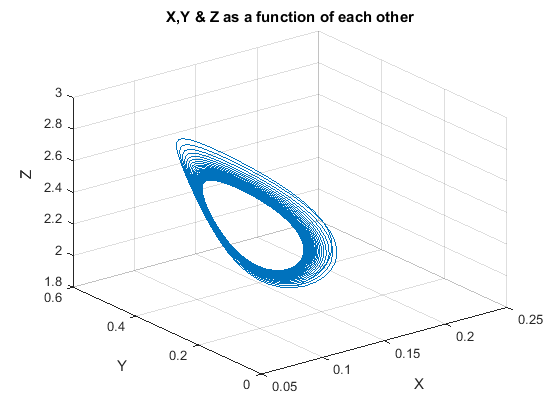
\includegraphics[width=\textwidth]{"../Miniprojet 2.0/Part A/A11.png}
	    \caption{Trajectories\\
	    The limit cycle is reached as the variations of $X(t)$, $Y(t)$ and $Z(t)$ become fixed : The trajectories converge, non-lineary (the distance between similar trajectories aren't regular) towards an ellipse (where the blue stripes accumulate)}
	\end{subfigure}
	~
	\begin{subfigure}[b]{0.5\textwidth}
	    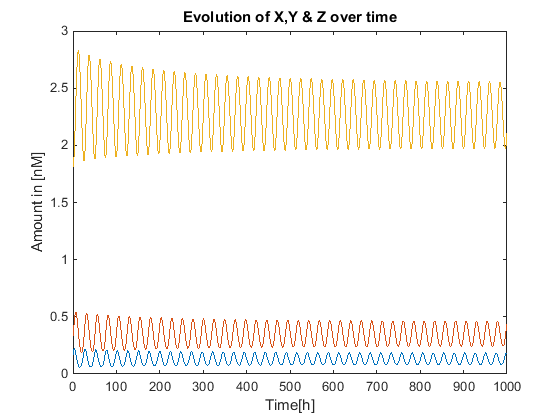
\includegraphics[width=\textwidth]{"../Miniprojet 2.0/Part A/A12.png}
	    \caption{Frequency spectrum \\
	    The amplitude of the three variations stabilize after a few hundred hours. The signal are not in phase but have the same, regular, frequencies.}
	\end{subfigure}
	\caption{\\Trajectories of $X(t)$, $Y(t)$ and $Z(t)$ when using initial conditions : $X_0 = $, $Y_0 = $, $Z_0 = $ \\ We observe on both graphs that $Z(t)$ has the bigger amplitude of variation whereas $X(t)$ and $Y(t)$ have small amplitudes. Additionaly, the convergence towards a single loop in (a) indicate that the frequencies of the signals are equal; this is illustrated as well in (b)
	}
    \end{figure*}

    \begin{figure*}
    \centering
	\begin{subfigure}[b]{0.32\textwidth}
	    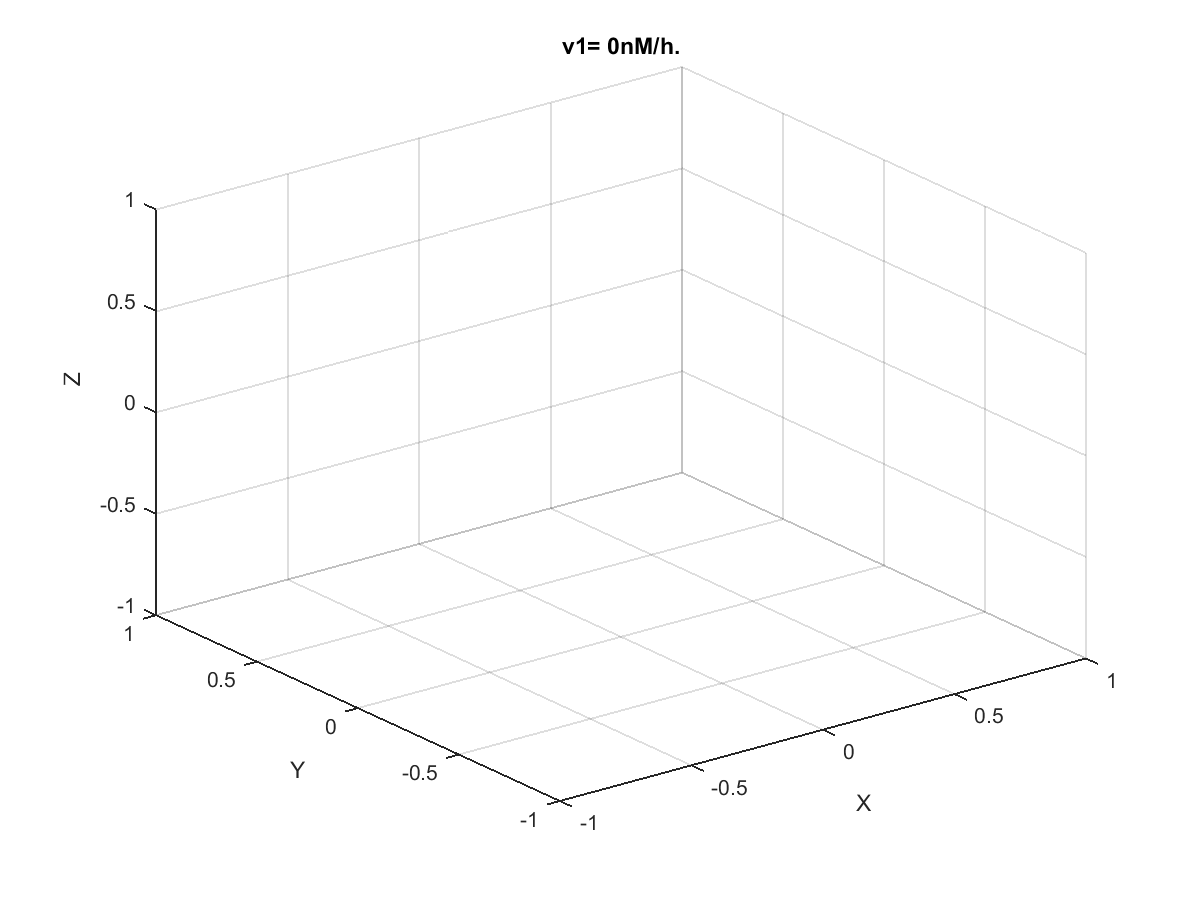
\includegraphics[width=\textwidth]{"../Miniprojet 2.0/Part A/LotsofthesameA/A-AA0.png}
	    \caption{$v_1$ = 0 nM/h}
	\end{subfigure}
	~ 
	\begin{subfigure}[b]{0.32\textwidth}
	    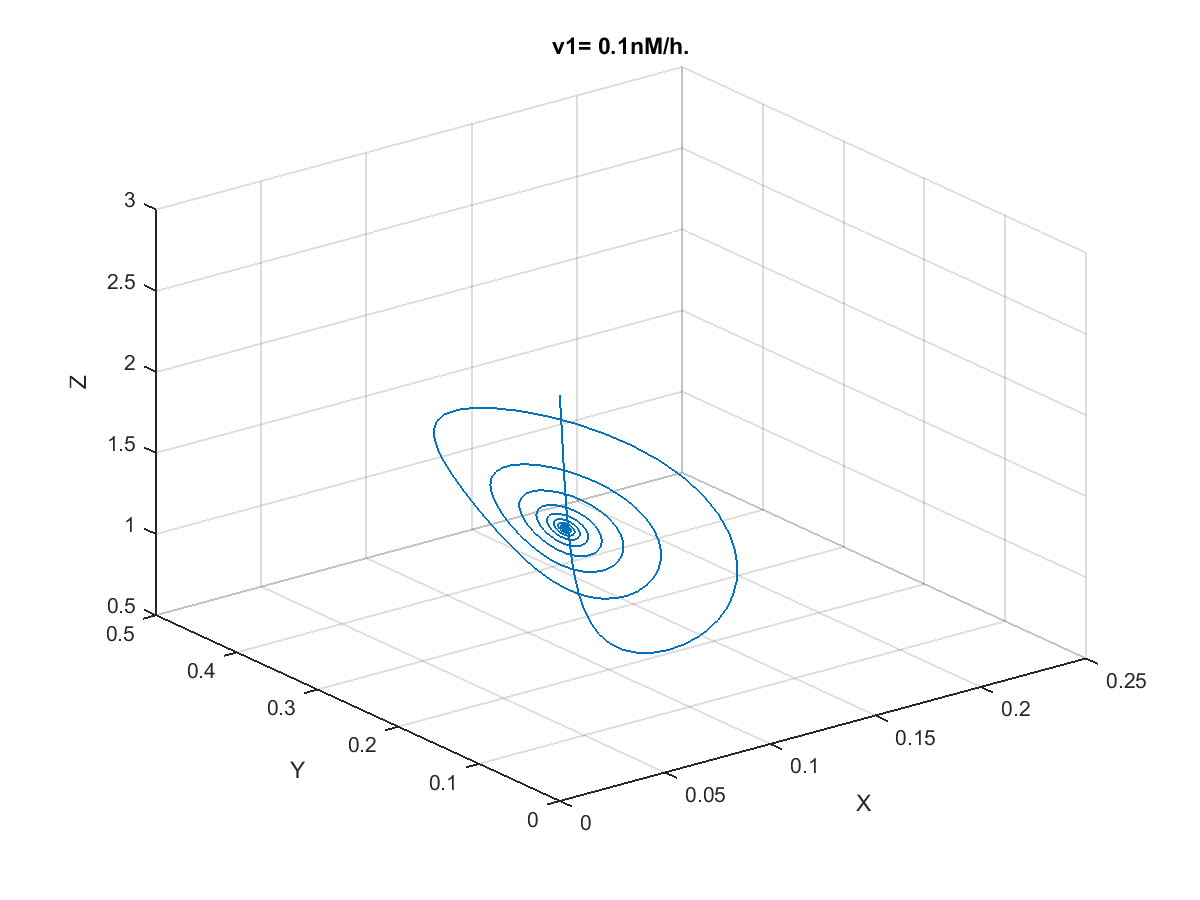
\includegraphics[width=\textwidth]{"../Miniprojet 2.0/Part A/LotsofthesameA/A-AA1.png}
	    \caption{$v_1$ = 1 nM/h}
	\end{subfigure}
	~ 
	\begin{subfigure}[b]{0.32\textwidth}
	    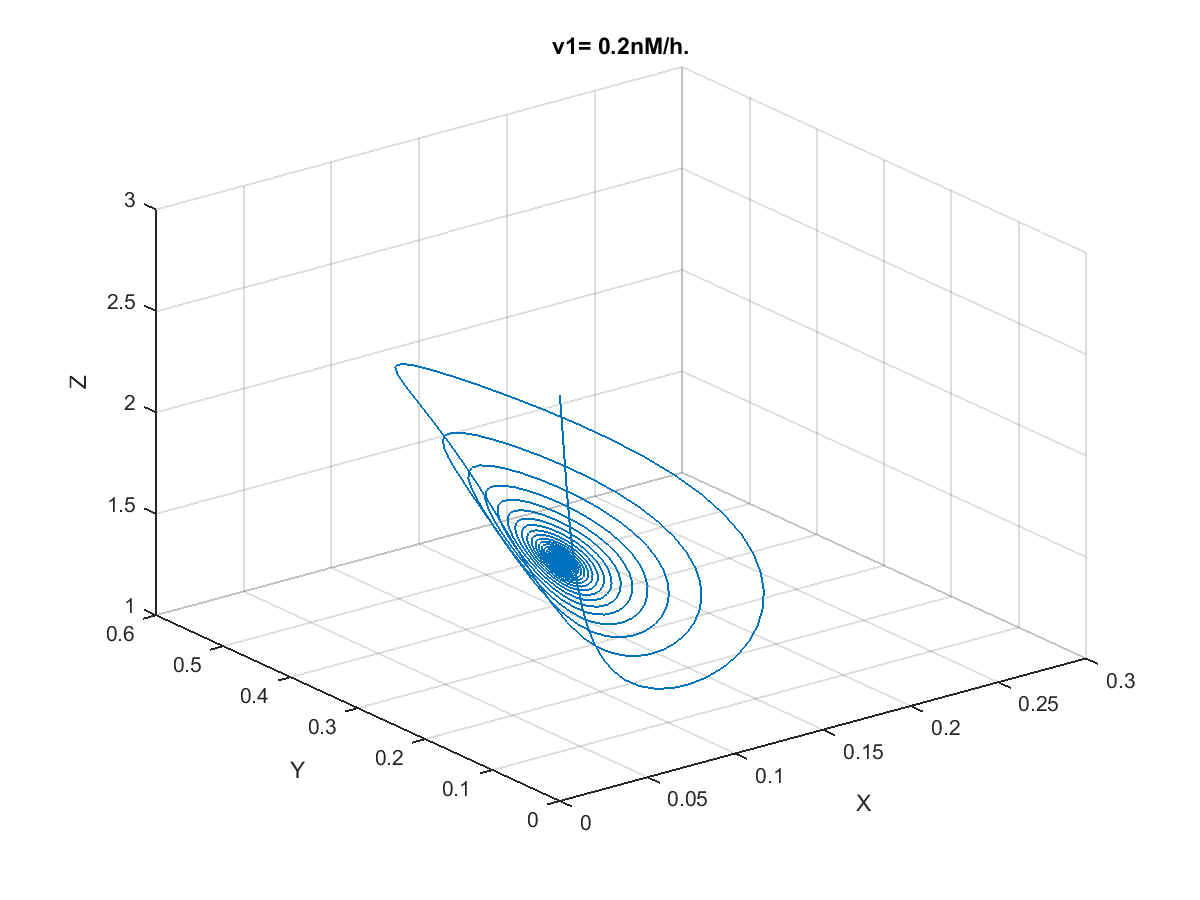
\includegraphics[width=\textwidth]{"../Miniprojet 2.0/Part A/LotsofthesameA/A-AA2.png}
	    \caption{$v_1$ = 2 nM/h}
	\end{subfigure}
	 
	\begin{subfigure}[b]{0.32\textwidth}
	    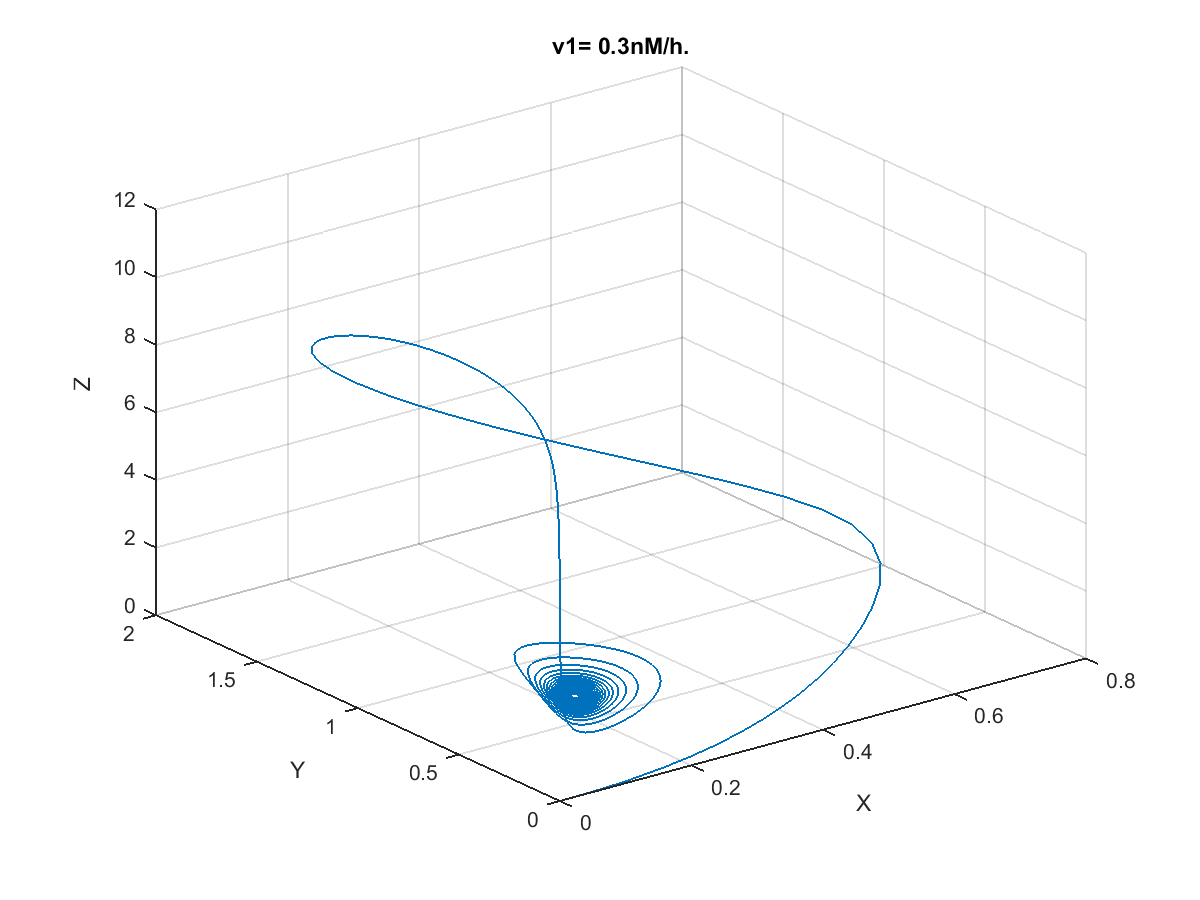
\includegraphics[width=\textwidth]{"../Miniprojet 2.0/Part A/LotsofthesameA/A-AA3.png}
	    \caption{$v_1$ = 3 nM/h}
	\end{subfigure}
	~ 
	\begin{subfigure}[b]{0.32\textwidth}
	    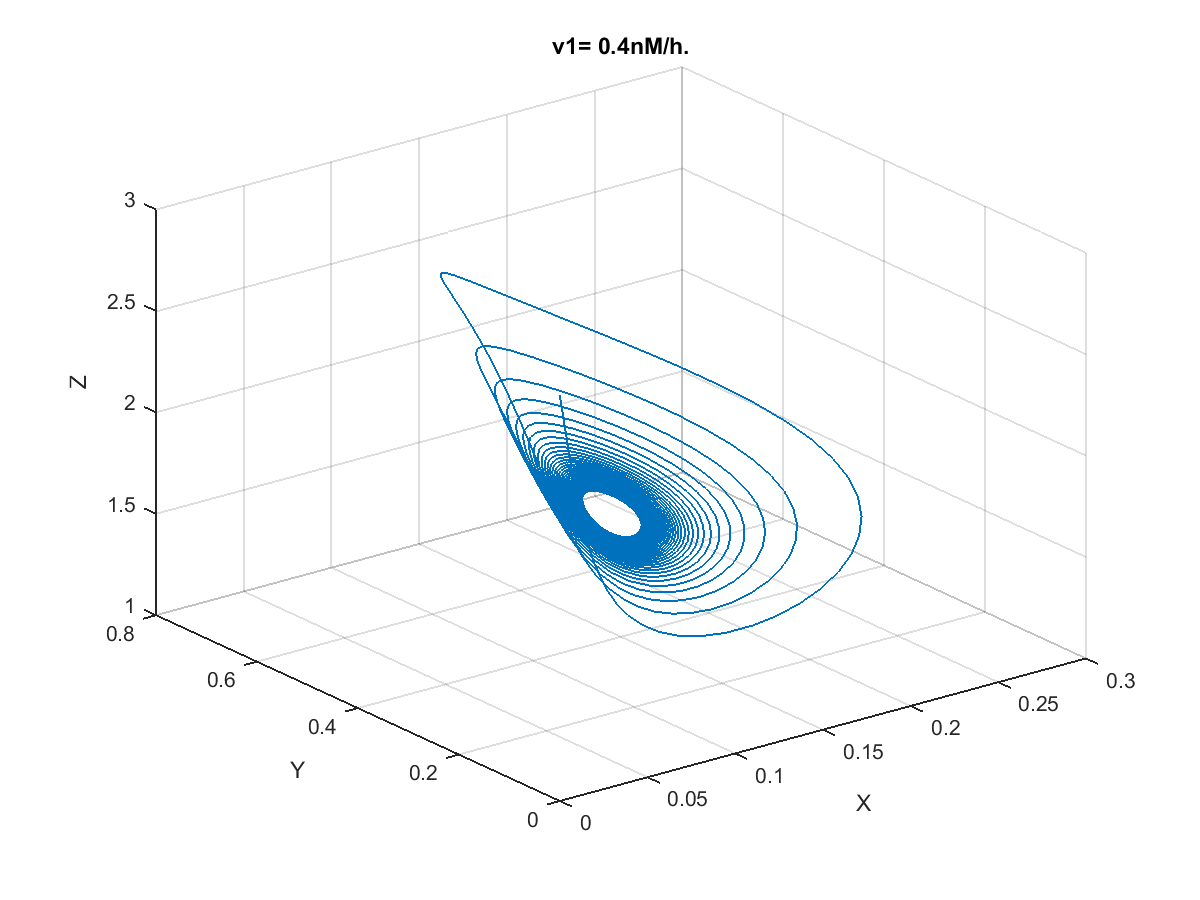
\includegraphics[width=\textwidth]{"../Miniprojet 2.0/Part A/LotsofthesameA/A-AA4.png}
	    \caption{$v_1$ = 4 nM/h}
	\end{subfigure}
	~
	\begin{subfigure}[b]{0.32\textwidth}
	    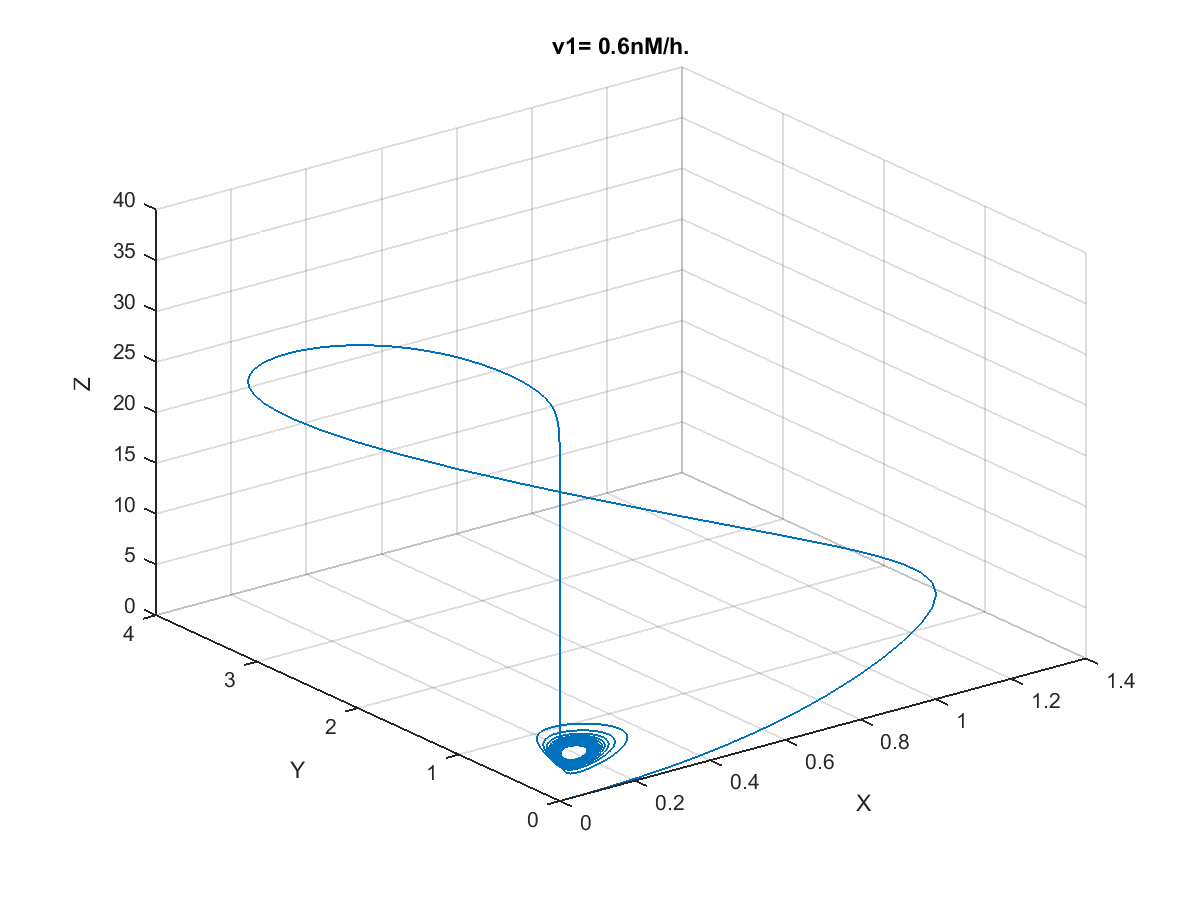
\includegraphics[width=\textwidth]{"../Miniprojet 2.0/Part A/LotsofthesameA/A-AA6.png}
	    \caption{$v_1$ = 6 nM/h}
	\end{subfigure}
	~ 
	\begin{subfigure}[b]{0.32\textwidth}
	    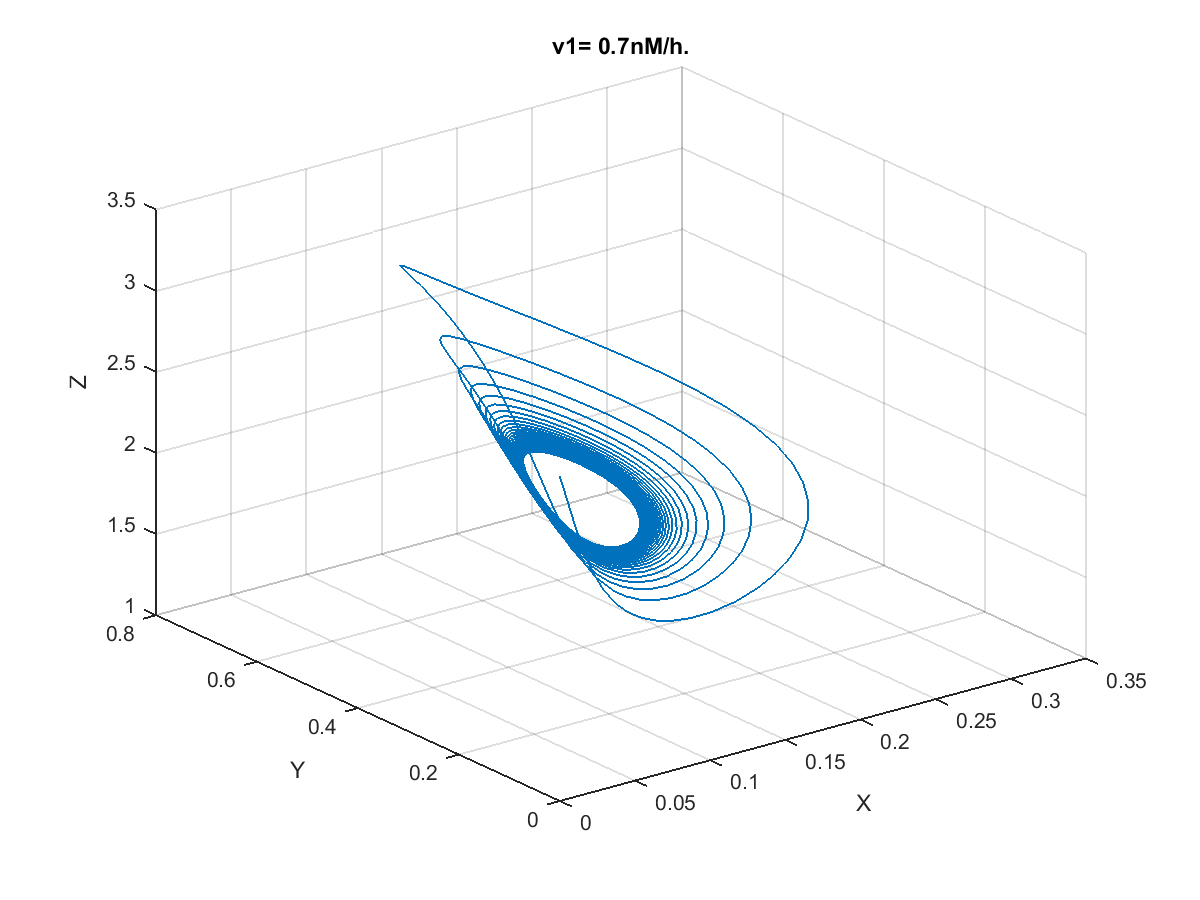
\includegraphics[width=\textwidth]{"../Miniprojet 2.0/Part A/LotsofthesameA/A-AA7.png}
	    \caption{$v_1$ = 8 nM/h}
	\end{subfigure}
	~
	\begin{subfigure}[b]{0.32\textwidth}
	    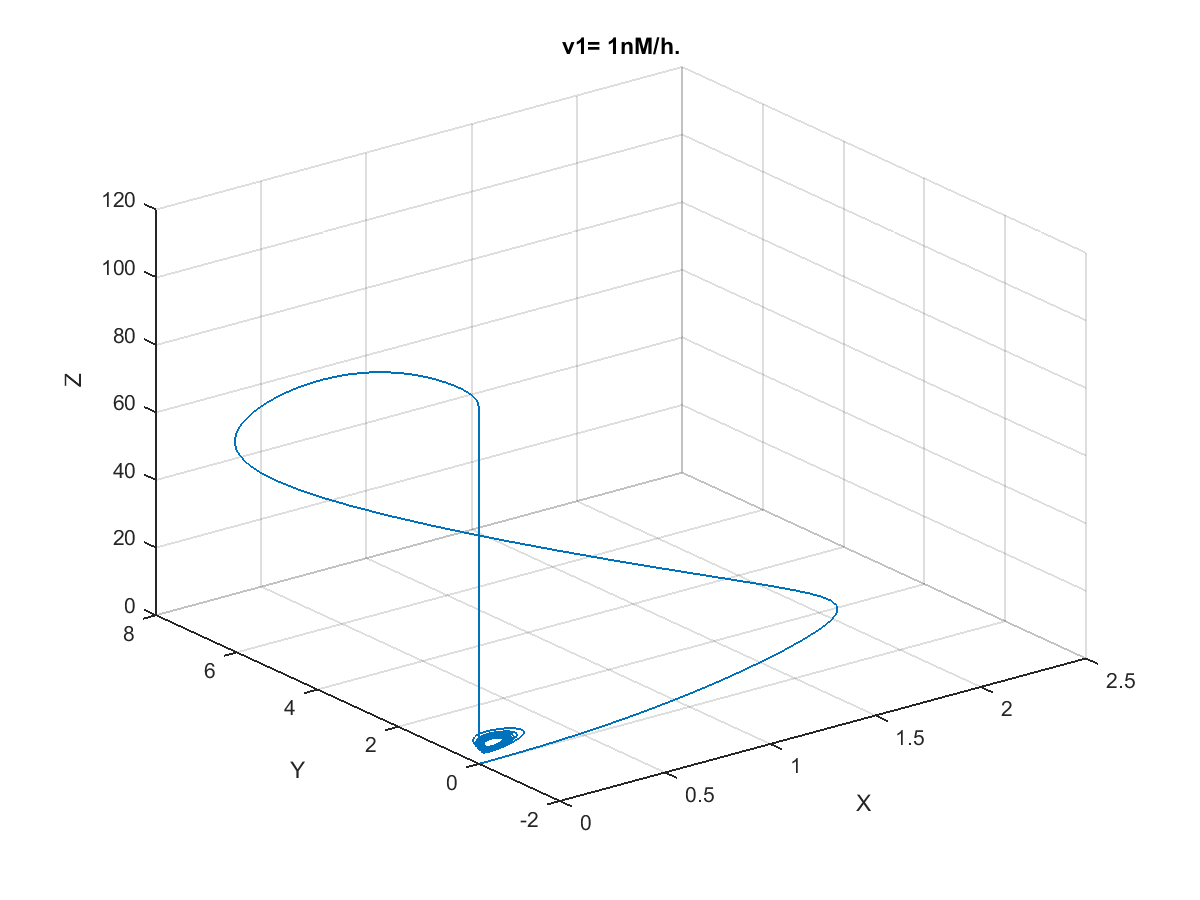
\includegraphics[width=\textwidth]{"../Miniprojet 2.0/Part A/LotsofthesameA/A-AA10.png}
	    \caption{$v_1$ = 10 nM/h}
	\end{subfigure}
	
	\caption{With nice initial conditions}
    \end{figure*}

    \begin{figure*}
    \centering
	\begin{subfigure}[b]{0.32\textwidth}
	    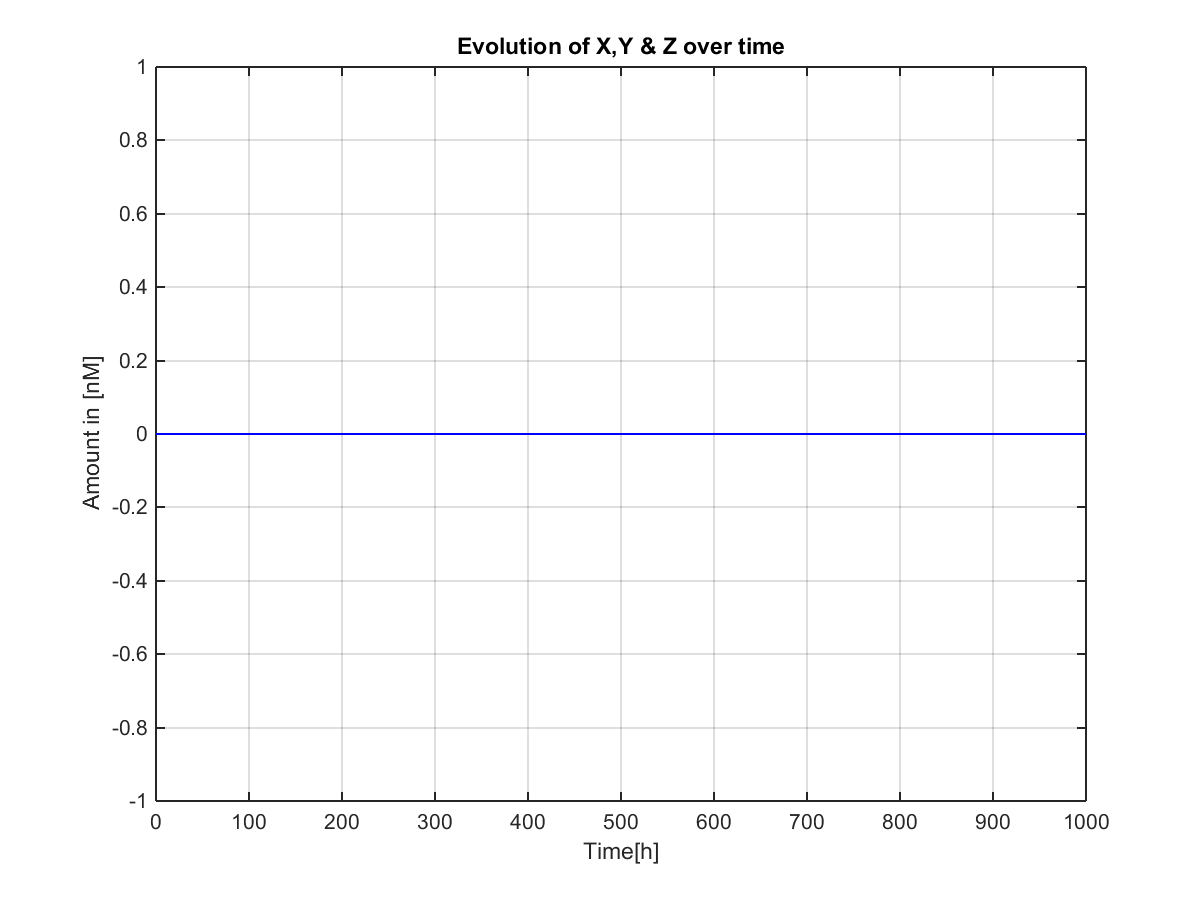
\includegraphics[width=\textwidth]{"../Miniprojet 2.0/Part A/LotsofthesameA/A-A0.png}
	    \caption{$v_1$ = 0 nM/h}
	    \end{subfigure}
	    ~ 
	    \begin{subfigure}[b]{0.32\textwidth}
	    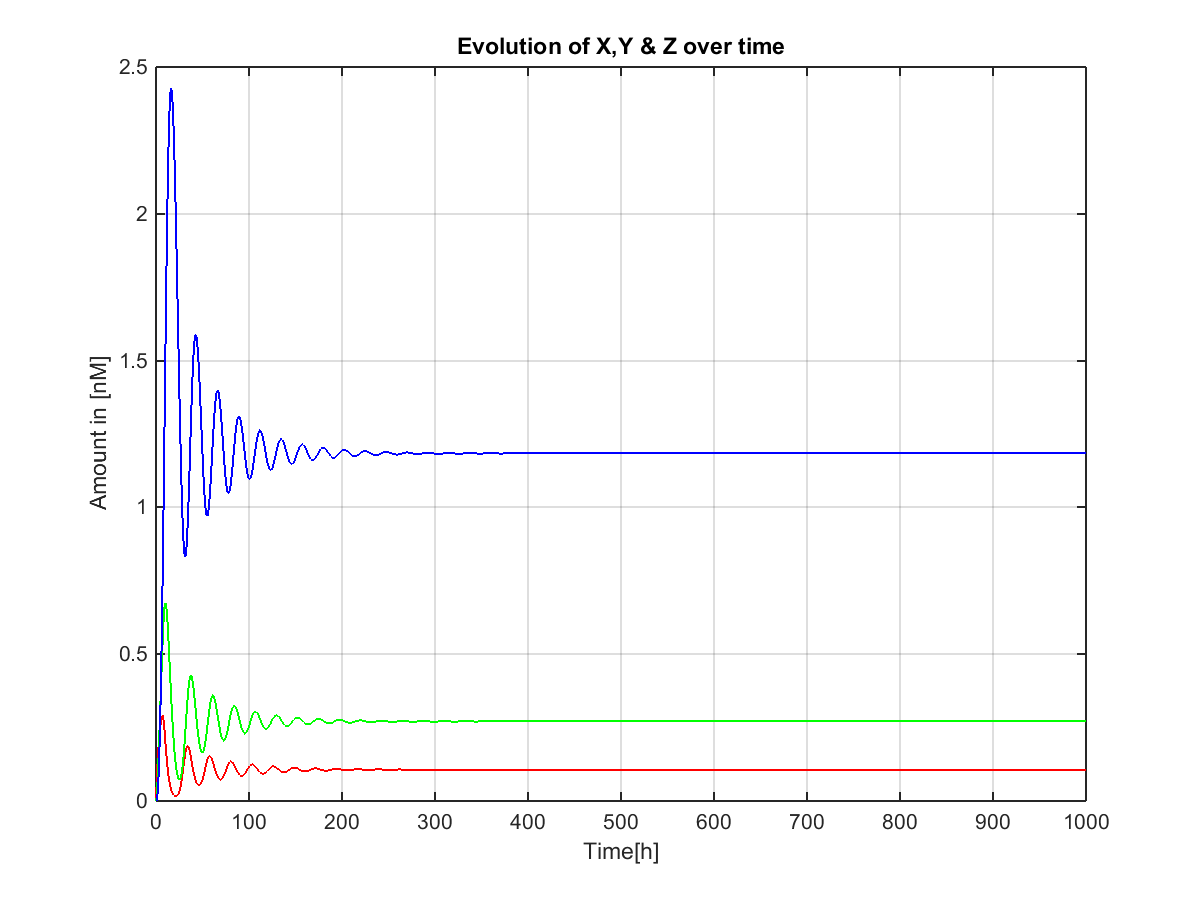
\includegraphics[width=\textwidth]{"../Miniprojet 2.0/Part A/LotsofthesameA/A-A1.png}
	    \caption{$v_1$ = 1 nM/h}
	    \end{subfigure}
	    ~ 
	\begin{subfigure}[b]{0.32\textwidth}
	    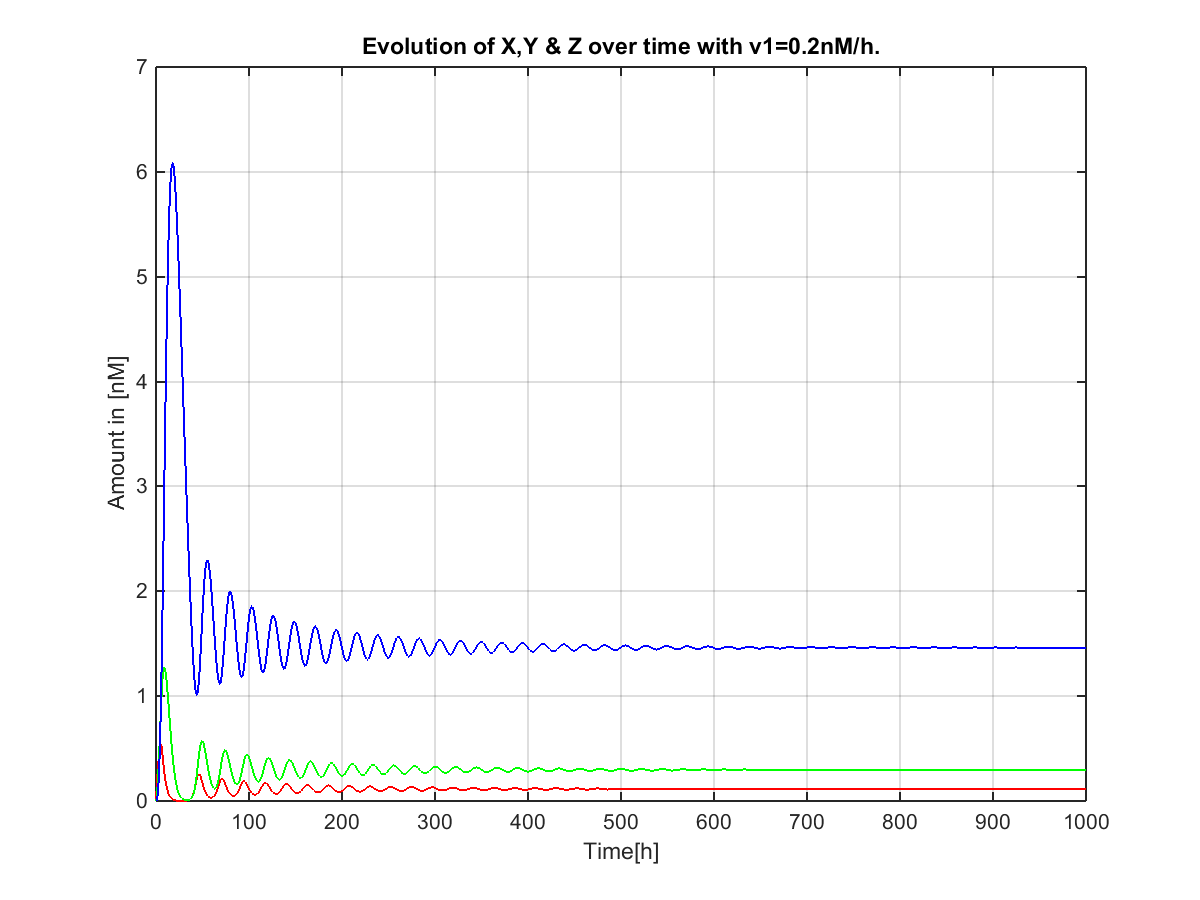
\includegraphics[width=\textwidth]{"../Miniprojet 2.0/Part A/LotsofthesameA/A-A2.png}
	    \caption{$v_1$ = 2 nM/h}
	\end{subfigure}
	 
	\begin{subfigure}[b]{0.32\textwidth}
	    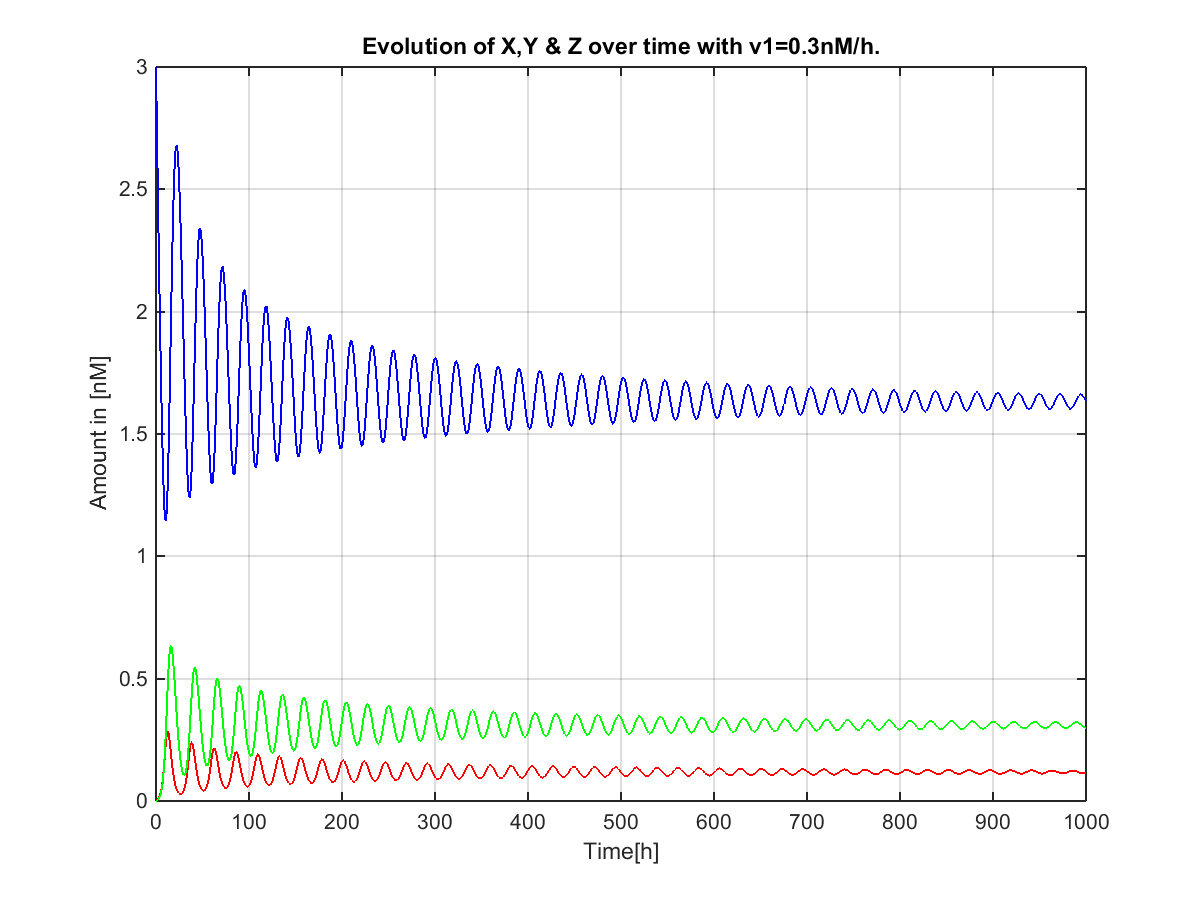
\includegraphics[width=\textwidth]{"../Miniprojet 2.0/Part A/LotsofthesameA/A-A3.png}
	    \caption{$v_1$ = 3 nM/h}
	\end{subfigure}
	~ 
	\begin{subfigure}[b]{0.32\textwidth}
	    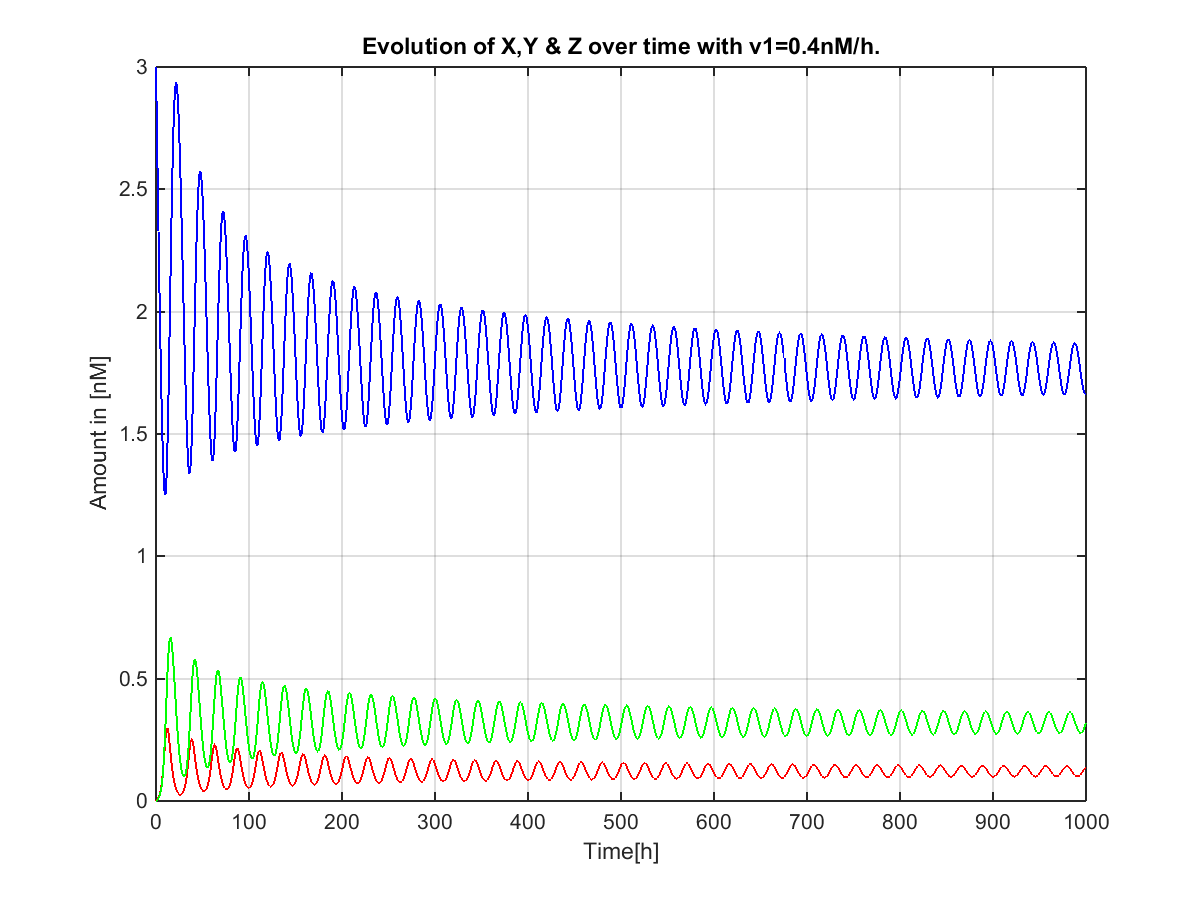
\includegraphics[width=\textwidth]{"../Miniprojet 2.0/Part A/LotsofthesameA/A-A4.png}
	    \caption{$v_1$ = 4 nM/h}
	\end{subfigure}
	~
	\begin{subfigure}[b]{0.32\textwidth}
	    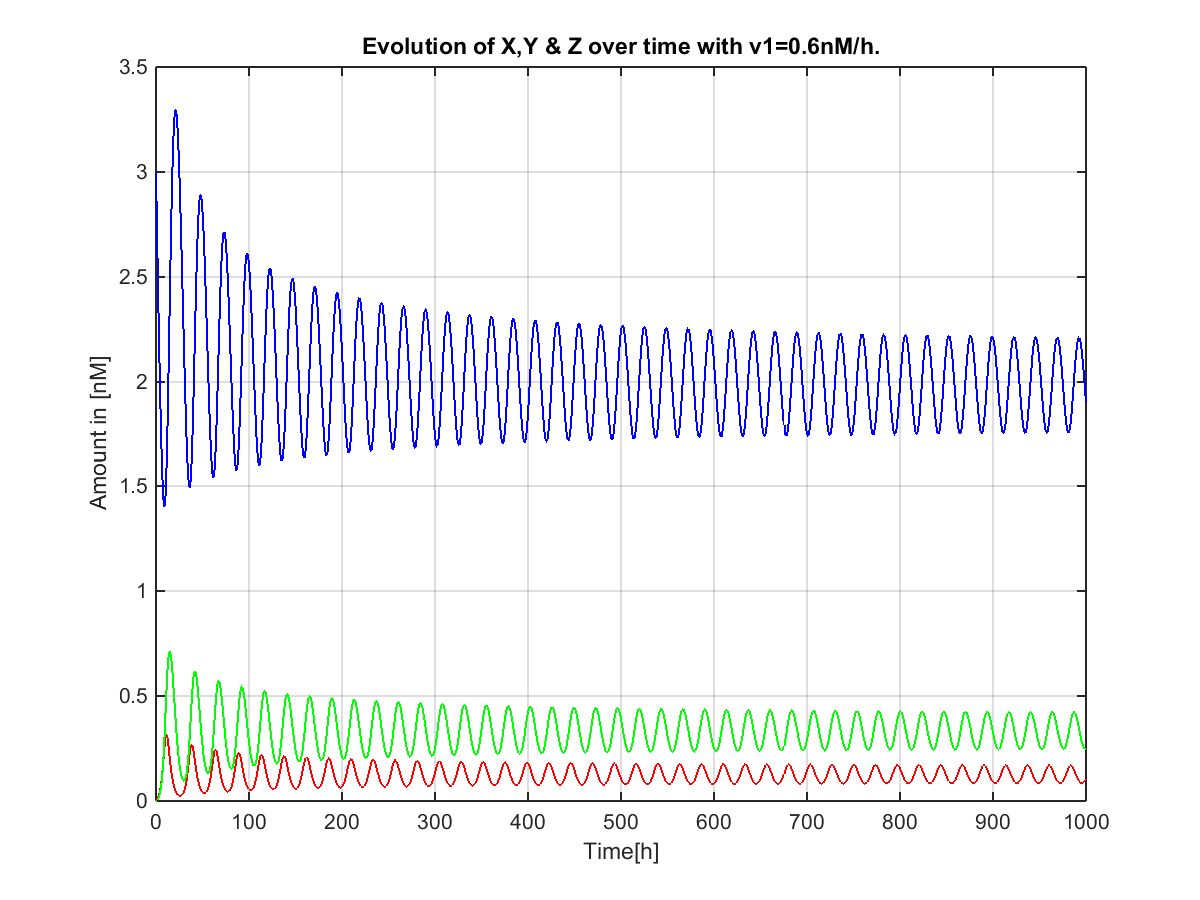
\includegraphics[width=\textwidth]{"../Miniprojet 2.0/Part A/LotsofthesameA/A-A6.png}
	    \caption{$v_1$ = 6 nM/h}
	\end{subfigure}
	~ 
	\begin{subfigure}[b]{0.32\textwidth}
	    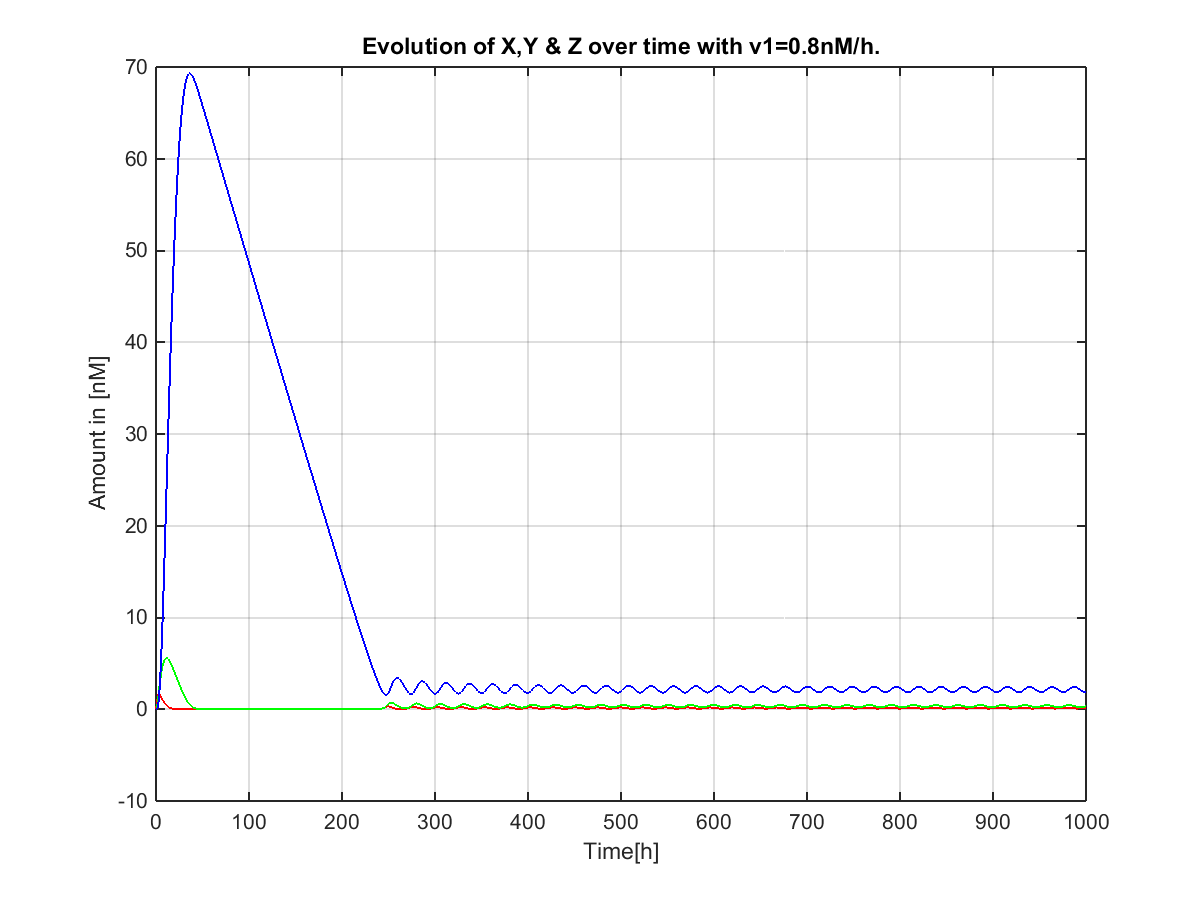
\includegraphics[width=\textwidth]{"../Miniprojet 2.0/Part A/LotsofthesameA/A-A8.png}
	    \caption{$v_1$ = 8 nM/h}
	\end{subfigure}
	~
	\begin{subfigure}[b]{0.32\textwidth}
	    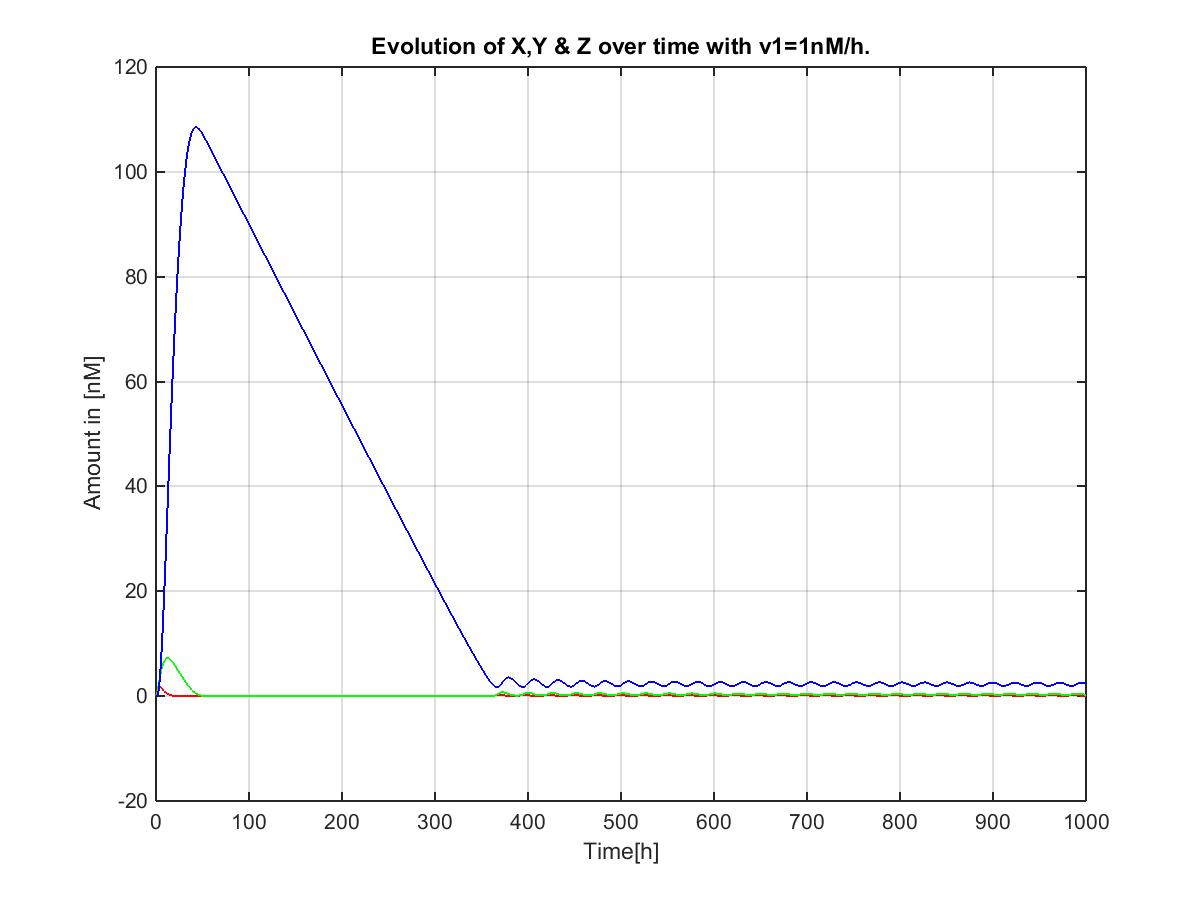
\includegraphics[width=\textwidth]{"../Miniprojet 2.0/Part A/LotsofthesameA/A-A10.png}
	    \caption{$v_1$ = 10 nM/h}
	\end{subfigure}

	\caption{With nice initial conditions}
    \end{figure*}

    \begin{figure*}
	\centering
	    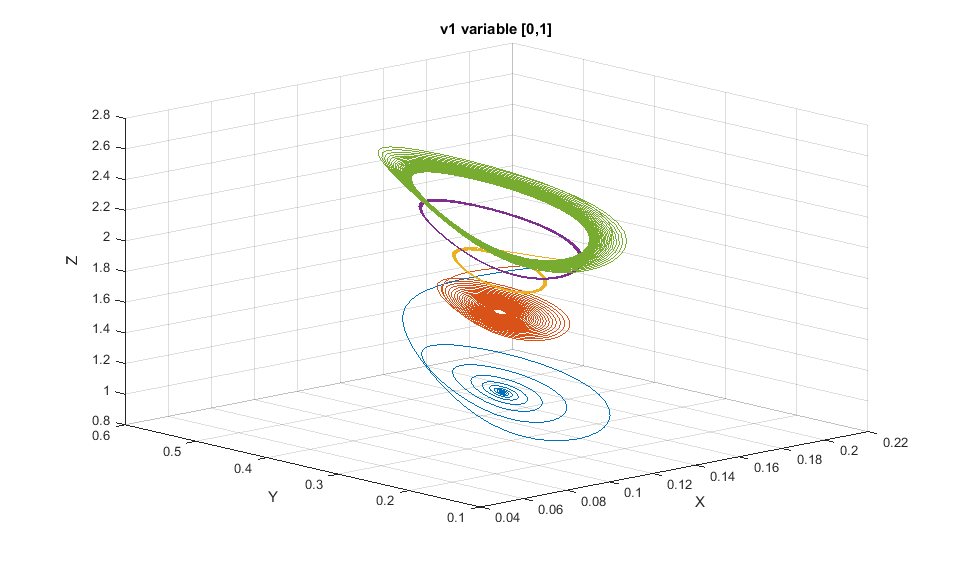
\includegraphics[width=0.5\textwidth]{"../Miniprojet 2.0/Part A/A2.png}
	    \caption{$v_1$ = \cyan{0.1}/\red{0.3}/\orange{0.5}/\purple{0.7}/\green{0.9} nM/h}
    \end{figure*}

    \begin{figure*}
	\centering
	    \begin{subfigure}[b]{0.45\textwidth}
		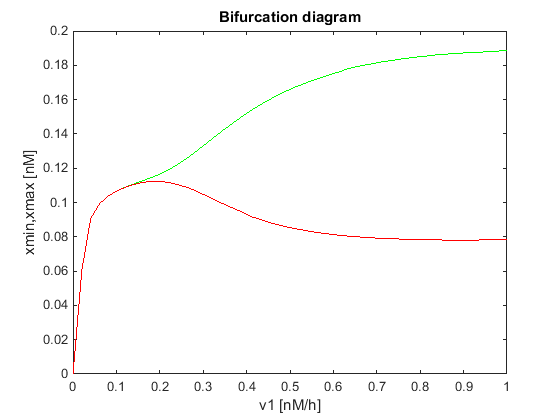
\includegraphics[width=\textwidth]{"../Miniprojet 2.0/Part A/Bifurcation.png}
		\caption{at $h_{max}=1000$}
	    \end{subfigure}
	     ~ 
	    \begin{subfigure}[b]{0.45\textwidth}
		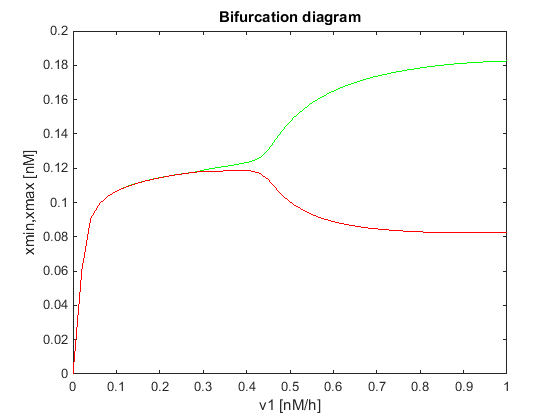
\includegraphics[width=\textwidth]{"../Miniprojet 2.0/Part A/Bifurcation10000.png}
		\caption{at $h_{max}=10000$}
	    \end{subfigure}
	    \caption{Bifurcation Diagram\\ plotted at time intervals : $[9/10; 1]$ of $h_{max}$}
    \end{figure*}

\end{document}
